\documentclass[12pt,vi]{mitthesis}
% \documentclass[12pt,vi,twoside]{mitthesis}
%%
%%  If you want your thesis copyright to you instead of MIT, use the
%%  ``vi'' option, as above.
%%
%\documentclass[12pt,twoside,leftblank]{mitthesis}
%%
%% If you want blank pages before new chapters to be labelled ``This
%% Page Intentionally Left Blank'', use the ``leftblank'' option, as
%% above. 

% \documentclass[12pt,twoside]{mitthesis}
\usepackage{lgrind}
%% These have been added at the request of the MIT Libraries, because
%% some PDF conversions mess up the ligatures.  -LB, 1/22/2014
% \usepackage{cmap}
\usepackage[T1]{fontenc}
\usepackage{xcolor}
\usepackage[version=4,arrows=pgf]{mhchem}
\usepackage[
    backend=biber,
    style=apa
    % style=authoryear
]{biblatex}
\addbibresource{reference.bib}
\usepackage{hyperref}
\usepackage{multirow}
\usepackage{subcaption}
% \usepackage[mathletters]{ucs}
% \usepackage[utf8x]{inputenc}
% \usepackage{unicode-math}
% \usepackage[letterpaper]{geometry}
\usepackage{unicode-math}
% \usepackage{xunicode}
\usepackage{minted}
\usepackage{fontspec}
% \setmonofont{FreeMono}
\usepackage{tikz}
\usetikzlibrary{positioning,arrows}
\usepackage{svg}
\usepackage[customcolors]{hf-tikz}
\usepackage{pgfplots}
\pgfplotsset{width=\textwidth,compat=1.9} 

\pagestyle{plain}

%% This bit allows you to either specify only the files which you wish to
%% process, or `all' to process all files which you \include.
%% Krishna Sethuraman (1990).

%\typein [\files]{Enter file names to process, (chap1,chap2 ...), or `all' to process all files:}
\def\all{all}
\ifx\files\all \typeout{Including all files.} \else %\typeout{Including only \files.} \includeonly{\files} \fi

\begin{document}

\pagenumbering{roman}
% -*-latex-*-
% 
% For questions, comments, concerns or complaints:
% thesis@mit.edu
% 
%
% $Log: cover.tex,v $
% Revision 1.9  2019/08/06 14:18:15  cmalin
% Replaced sample content with non-specific text.
%
% Revision 1.8  2008/05/13 15:02:15  jdreed
% Degree month is June, not May.  Added note about prevdegrees.
% Arthur Smith's title updated
%
% Revision 1.7  2001/02/08 18:53:16  boojum
% changed some \newpages to \cleardoublepages
%
% Revision 1.6  1999/10/21 14:49:31  boojum
% changed comment referring to documentstyle
%
% Revision 1.5  1999/10/21 14:39:04  boojum
% *** empty log message ***
%
% Revision 1.4  1997/04/18  17:54:10  othomas
% added page numbers on abstract and cover, and made 1 abstract
% page the default rather than 2.  (anne hunter tells me this
% is the new institute standard.)
%
% Revision 1.4  1997/04/18  17:54:10  othomas
% added page numbers on abstract and cover, and made 1 abstract
% page the default rather than 2.  (anne hunter tells me this
% is the new institute standard.)
%
% Revision 1.3  93/05/17  17:06:29  starflt
% Added acknowledgements section (suggested by tompalka)
% 
% Revision 1.2  92/04/22  13:13:13  epeisach
% Fixes for 1991 course 6 requirements
% Phrase "and to grant others the right to do so" has been added to 
% permission clause
% Second copy of abstract is not counted as separate pages so numbering works
% out
% 
% Revision 1.1  92/04/22  13:08:20  epeisach

% NOTE:
% These templates make an effort to conform to the MIT Thesis specifications,
% however the specifications can change. We recommend that you verify the
% layout of your title page with your thesis advisor and/or the MIT 
% Libraries before printing your final copy.
\title{A Chemical Reaction Network Approach for Modeling Pollutant Formation in Large Industrial Furnaces 
% \\ (Dutch title: Een Chemische-Reactie-Network Benadering voor het Modelleren van het Vormen van Verontreinigende in Grote Industriele Ovens)
}

\author{Bowen Shuchai Zhu}
% If you wish to list your previous degrees on the cover page, use the 
% previous degrees command:
%       \prevdegrees{A.A., Harvard University (1985)}
% You can use the \\ command to list multiple previous degrees
%       \prevdegrees{B.S., University of California (1978) \\
%                    S.M., Massachusetts Institute of Technology (1981)}
\department{Faculty of Electrical Engineering, Mathematics and Computer Science}

% If the thesis is for two degrees simultaneously, list them both
% separated by \and like this:
% \degree{Doctor of Philosophy \and Master of Science}
\degree{Bachelor of Science in Applied Mathematics 
\and Bachelor of Science in Computer Science and Engineering}

% As of the 2007-08 academic year, valid degree months are September, 
% February, or June.  The default is June.
\degreemonth{July}
\degreeyear{2021}
\thesisdate{July 2, 2021}

%% By default, the thesis will be copyrighted to MIT.  If you need to copyright
%% the thesis to yourself, just specify the `vi' documentclass option.  If for
%% some reason you want to exactly specify the copyright notice text, you can
%% use the \copyrightnoticetext command.  
%\copyrightnoticetext{\copyright IBM, 1990.  Do not open till Xmas.}

% If there is more than one supervisor, use the \supervisor command
% once for each.
\supervisor{Domenico J. P. Lahaye}{Associate Professor}

\committee{Johan L. A. Dubbeldam}{Associate Professor}
\committee{Matthias M\"oller}{Associate Professor}

% This is the department committee chairman, not the thesis committee
% chairman.  You should replace this with your Department's Committee
% Chairman.
% \chairman{Johan L. A. Dubbeldam}{Associate Professor}

% Make the titlepage based on the above information.  If you need
% something special and can't use the standard form, you can specify
% the exact text of the titlepage yourself.  Put it in a titlepage
% environment and leave blank lines where you want vertical space.
% The spaces will be adjusted to fill the entire page.  The dotted
% lines for the signatures are made with the \signature command.
\maketitle

% The abstractpage environment sets up everything on the page except
% the text itself.  The title and other header material are put at the
% top of the page, and the supervisors are listed at the bottom.  A
% new page is begun both before and after.  Of course, an abstract may
% be more than one page itself.  If you need more control over the
% format of the page, you can use the abstract environment, which puts
% the word "Abstract" at the beginning and single spaces its text.

%% You can either \input (*not* \include) your abstract file, or you can put
%% the text of the abstract directly between the \begin{abstractpage} and
%% \end{abstractpage} commands.

% First copy: start a new page, and save the page number.
\cleardoublepage
% Uncomment the next line if you do NOT want a page number on your
% abstract and acknowledgments pages.
% \pagestyle{empty}
% \setcounter{savepage}{\thepage}
\begin{abstractpage}
The chemical reaction network (CRN) approach is a practical tool for precisely predicting the species concentration in combustion processes with low computational cost. This work examines the capability of the emerging Julia programming language and its ecosystem in solving large CRNs. The packages DifferentialEquations.jl and ModelingToolkit.jl are employed to defining and solving stiff ordinary differential equations, for which the Rosenbrock and ESDIRK implicit time-integration methods with the GMRES linear solver are used. The graph structure of reaction networks is constructed by LightGraphs.jl and SimpleWeightedGraphs.jl. The differential equation solver and the graph data structure are connected via NetworkDynamics.jl. It is concluded that Julia is a competent tool for the CRN approach. Julia is capable of simulating pollutant formation in large reaction networks within reasonable time.
\end{abstractpage}

% Additional copy: start a new page, and reset the page number.  This way,
% the second copy of the abstract is not counted as separate pages.
% Uncomment the next 6 lines if you need two copies of the abstract
% page.
% \setcounter{page}{\thesavepage}
% \begin{abstractpage}
% \input{abstract}
% \end{abstractpage}

\cleardoublepage

% \section*{Acknowledgments}

% This is the acknowledgements section. You should replace this with your own acknowledgements.

% {\large \color{red} TODO}

%%%%%%%%%%%%%%%%%%%%%%%%%%%%%%%%%%%%%%%%%%%%%%%%%%%%%%%%%%%%%%%%%%%%%%
% -*-latex-*-

% Some departments (e.g. 5) require an additional signature page.  See
% signature.tex for more information and uncomment the following line if
% applicable.
% \include{signature}
\pagestyle{plain}
  % -*- Mode:TeX -*-
%% This file simply contains the commands that actually generate the table of
%% contents and lists of figures and tables.  You can omit any or all of
%% these files by simply taking out the appropriate command.  For more
%% information on these files, see appendix C.3.3 of the LaTeX manual. 
\tableofcontents
% \newpage
% \listoffigures
% \newpage
% \listoftables


\pagenumbering{arabic}
\chapter{Introduction} 

To move an aircraft, a propulsion system is needed to create thrust. Different engines develop thrust in different ways, but all depend on burning fuels. The chemical process of burning a fuel is called combustion. In such a process, oxygen reacts rapidly with a fuel which can be solid, liquid, or gas. During combustion, new chemical substances, called exhaust, are produced, most of which are water (\ce{H2O}, hydrogen + oxygen) and carbon dioxide (\ce{CO2}, carbon + oxygen). However, the emission of by-products are inevitable such as nitrogen oxides (\ce{NO_x}, nitrogen + oxygen) since nitrogen constitutes around 78\% of air besides the presence of dioxygen. Nitric oxide (\ce{NO}) and nitrogen dioxide (\ce{NO2}) contribute to the formation of smog and acid rain and badly influences ozone. Another air pollutant gas, carbon monoxide (\ce{CO}), also plays roles affecting climate change. Therefore, adequate tools are required for estimating emissions. This thesis aims at developing a simulator written in the Julia programming language following the chemical reactor network approach to model the formation of pollutants. In this project, we focus on the combustion of natural gas with methane (\ce{CH4}) as its main component\footnote{we neglect here the presence of higher alkanes such as propane (\ce{C3H8}) and butane (\ce{C4H10}).} in large industrial furnaces. 

An overview is given in this chapter. Chapter~\ref{ch:combustion} further describes the combustion of methane and its reaction network in furnaces. Chapter~\ref{ch:julia} introduces the ecosystem of the Julia programming language. {\large \color{red} TODO}
\chapter{Combustion} \label{ch:combustion}

Combustion of gaseous fuels is the combined process of the mixing of fuel (methane) and oxidizer (oxygen) with transport of chemical species in a flow. To simulate combustion, we model the chemical reactions aiming at a sufficiently accurate description of the formation of major and minor species during the chemical reactions. The computational domain that represents the furnace is subdivided into subdomains (containers, vessels or reactors). The dimension of the subdomain is large compared to the typical dimension of a cell required to resolve the flow. These subdomains are interconnected by the flow on mass leaving one reactor and entering the other reactor. The furnace is represented as a chemical reaction network. A chemical reactor network consists of nodes and edges. The nodes and edges represent chemical reactors (subdomains) and interconnecting pipes, respectively. As for chemical reaction, we will consider the combustion of methane and ambient air at atmospheric pressure and constant volume. To alleviate computational cost, the representation of the flow is simplified. 

\section{Basic mechanism of methane combustion} \label{sec:methane_mechanism}

The natural gas we consider here is a fuel primarily consisting of methane (\ce{CH4}). When one methane molecule meets two oxygen molecules with sufficient heat, they start to react and then one molecule of carbon dioxide and two molecules of water are formed.

\begin{equation}
    \ce{CH4 + 2 O2 -> CO2 + 2 H2O}.
\end{equation}

The rate of reaction is governed by the formulas

\begin{subequations}
\begin{align}
    \frac{\mathrm d [\ce{CH4}]}{\mathrm d t} &= - k , \\
    \frac{\mathrm d [\ce{O2}]}{\mathrm d t} &= - 2k , \\
    \frac{\mathrm d [\ce{CO2}]}{\mathrm d t} &= k , \\
    \frac{\mathrm d [\ce{H2O}]}{\mathrm d t} &= 2k ,
\end{align}
\end{subequations}
\begin{equation}
    k = A T^\beta \exp(- E_a / R T) [\ce{CH4}]^{n_{\ce{CH4}}} [\ce{O2}]^{n_{\ce{O2}}}, 
\end{equation}
where $[ \, \cdot \,]$ means the concentration of a species, $k$ is the rate coefficients, $E_a$ is the activation energy, $R$ is the gas constant, $T$ is temperature and $\beta$ is the temperature exponent.  This relation is also known as the Arrhenius law, in which the reaction rate depends on the temperature through the Arrhenius equation and the pressure through the influence of pressure on molecular space density which affects the species concentrations. 

Depending on the level of detail of the mechanism, the reaction of methane and oxygen may produce carbon dioxide and water in a single step. The reaction can also be expressed in two steps. See subsection~\ref{subsec:CO} for more details. 

\section{Pollutants}

Some products of combustion are harmful to the health of humans and other living beings and cause damage to the climate. The minor species, namely pollutants, of conventional combustion systems include \ce{CO}, \ce{UHC}, \ce{NO_x}, \ce{SO_x}. For the research to be conducted, \ce{CO} and \ce{NO_x} are relevant pollutants and are thus considered in the following.

\subsection{Carbon monoxide} \label{subsec:CO}

Carbon monoxide (\ce{CO}) is a colorless, odorless atmospheric pollutant mainly from the exhaust of incomplete combustion of fuels. Large CO pollution events can be observed from space over cities \parencite{COemmision}. Breathing air with high concentration of \ce{CO} leads to a reduced oxygen (\ce{O2}) transport in the blood stream to critical organs such as heart and brain \parencite{COpollution}.

The 2S\_CH4\_BFER scheme by \textcite{FRANZELLI2012621} accounts for six species (\ce{CH4}, \ce{O2}, \ce{N2}, \ce{CO}, \ce{CO2}, \ce{H2O}) and the following two reactions:
\begin{subequations} \label{re:CO}
\begin{align}
    \ce{CH4 + 1.5 O2 &-> CO + 2 H2O} \label{re:CO1} \\
    \ce{CO + 0.5 O2 &<=> CO2} , \label{re:CO2}
\end{align}
\end{subequations}
where the forward reaction rate for reactions \eqref{re:CO} are
\begin{subequations}
\begin{align}
    k_1 &= A_1 T^{\beta_1} \exp(-E_{a,1} / RT) [\ce{CH4}]^{n_{\ce{CH4}}} [\ce{O2}]^{n_{\ce{O2},1}} , \\
    k_2 &= A_2 T^{\beta_2} \exp(-E_{a,2} / RT) [\ce{CO}]^{n_{\ce{CO}}} [\ce{O2}]^{n_{\ce{O2},2}}.
\end{align}
\end{subequations}

The reaction parameters are summarized in table~\ref{tab:CO_k} \parencite{FRANZELLI2012621}.

\begin{table}[h!]
\centering
\begin{tabular}{| l l c l c |} 
 \hline
 Parameters & \multicolumn{2}{l}{\ce{CH4} oxidation \eqref{re:CO1}} & \multicolumn{2}{l|}{\ce{CO}-\ce{CO2} equilibrium \eqref{re:CO2}} \\
 \hline
 Activation energy $E_a$ & \multicolumn{2}{l}{$3.55 \times 10^4$} & \multicolumn{2}{l|}{$1.2 \times 10^4$} \\ 
 Temperature exponent $\beta$ & \multicolumn{2}{l}{0.0} & \multicolumn{2}{l|}{0.8} \\
 Pre-exponential factor $A$ & \multicolumn{2}{l}{$4.9 \times 10^9$} & \multicolumn{2}{l|}{$2 \times 10^8$} \\
 Reaction exponents & $n_{\ce{CH4}}$ & 0.50 & $n_{\ce{CO}}$ & 1.00 \\
  & $n_{\ce{O2},1}$ & 0.65 & $n_{\ce{O2},2}$ & 0.50 \\
 \hline
\end{tabular}
\caption{Reaction parameters for the 2S\_CH4\_BFER mechanism}
\label{tab:CO_k}
\end{table}



Furthermore, \textcite{JONES1988233} presented a four-step mechanism which could be useful for more accurate simulation.

\subsection{Nitrogen oxides}

Oxygen and nitrogen in general do not react at ambient temperatures due to lack of energy. But at high temperatures typically in internal combustion engines, they undergo an endothermic reaction producing various oxides of nitrogen (\ce{NO_x}). 

Nitrogen oxides mainly result in two forms of air pollution. In the presence of sunlight, \ce{NO_x} reacts with volatile organic compounds (VOCs) yielding photochemical smog. People with lung diseases and people who work or exercise outside are particularly susceptible to adverse effects of smog such as damage to lung tissue and reduction in lung function \parencite{NOlung}. Furthermore, \ce{NO_x} generates nitric acid and acid rain by reacting in certain environments.

The primary sources of \ce{NO_x} in combustion processes are dominated by the thermal \ce{NO} formation, also well known as the Zel'dovich mechanism \parencite{NO_Zeldovich}. The reaction mechanism consists of two chain reactions:
\begin{subequations} \label{re:NO}
\begin{gather}
    \ce{O + N2 <=>[$k_1$] NO + N} \label{re:NO_1} \\
    \ce{N + O2 <=>[$k_2$] NO + O} \label{re:NO_2} 
\end{gather}
which can be extended by adding the reaction
\begin{equation}
    \ce{N + OH <=>[$k_3$] NO + H}. \label{re:NO_3} 
\end{equation}
\end{subequations}

The forward and backward reaction rate constants for reactions \eqref{re:NO} are given in table~\ref{tab:NO_k} \parencite[p.~171]{NO_k}.

\begin{table}[ht!]
\centering
\begin{tabular}{|l l l|} 
 \hline
 \multirow{2}{*}{Reaction} & Forward reaction rate & Backward reaction rate \\
 & coefficients ($\mathrm m^3$/(kmol)(s)) & coefficients ($\mathrm m^3$/(kmol)(s)) \\
 \hline
 \ref{re:NO_1} & $k_{1f} = 1.8 \times 10^{11} \exp(-38370/T)$ & $k_{1b} = 3.8 \times 10^{10} \exp(-425/T)$ \\ 
 \ref{re:NO_2} & $k_{2f} = 1.8 \times 10^7 \exp(-4680/T)$ & $k_{2b} = 3.8 \times 10^6 \exp(-20820/T)$ \\ 
 \ref{re:NO_3} & $k_{3f} = 7.1 \times 10^{10} \exp(-450/T)$ & $k_{3b} = 1.7 \times 10^{11} \exp(-24560/T)$ \\ 
 \hline
\end{tabular}
\caption{Reaction rates for the extended Zel'dovich mechanism}
\label{tab:NO_k}
\end{table}

Note that reaction~\eqref{re:NO_1} has a very high activation energy ($E_a = 38370 R = 38370 \times 8.3145 = 319027 \, \mathrm{kJ/mol}$) by contrast. Reactions~\eqref{re:NO_2} and \eqref{re:NO_3} have been found to be much faster than reaction~\eqref{re:NO_1}. If simulation timescale is sufficiently long, one can assume that \ce{N2}, \ce{O2}, \ce{O} and \ce{OH} concentrations are at equilibrium and \ce{N} atoms are in steady state, which simplifies the calculation of the \ce{NO} formation. The reverse reaction can be further neglected by assuming that the \ce{NO} concentration is much less than its equilibrium value. So the rate expression is:
\begin{subequations}
\begin{align}
    \frac{\mathrm d [\ce{NO}]}{\mathrm d t} &= k_{1f} [\ce{O}] [\ce{N2}] + k_{2f} [\ce{N}] [\ce{O2}] + k_{3f} [\ce{N}] [\ce{OH}] \\
    \frac{\mathrm d [\ce{N}]}{\mathrm d t} &= k_{1f} [\ce{O}] [\ce{N2}] - k_{2f} [\ce{N}] [\ce{O2}] - k_{3f} [\ce{N}] [\ce{OH}] = 0 \\
    \implies \quad \frac{\mathrm d [\ce{NO}]}{\mathrm d t} &= 2 k_{1f} [\ce{O}] [\ce{N2}]
\end{align}
\end{subequations}

\section{Chemical reaction network} \label{sec:CRN}

Computer-based simulation techniques are commonly used by gas turbine manufacturers in the field of new combustor designs. To describe pollutant formation accurately, around $10^2$ species and $10^3$ reactions must be considered besides the simplest fuels. Currently, it is too computationally expensive to include all phenomena of importance in a single accurate computational fluid dynamics (CFD) simulation for a combustion system. For the sake of compensating detailed chemistry, the chemical reaction network (CRN) approach has been developed with the cost of reduced treatment of fluid dynamics \parencite{CRN}. A trend can be seen that emission simulation may move from the high-budget CFD approaches to CRN approaches where a network of idealized chemical reactors simplifies the computation for combustion modelling \parencite{CRN_review}.

The CRN modelling approach is used for modelling combustion processes. The inner combustor space is divided into several regions. The deviation of physical and chemical properties is relatively small such that each region can be modelled as a node with detailed chemistry in the chemical reaction network. The physical flow of substances is captured by edges connecting nodes.
\chapter{ Julia programming language} \label{ch:julia}

{\large \color{red} TODO}

\section{DifferentialEquations.jl}

\parencite{DifferentialEquations.jl}

\section{ModelingToolkit.jl}

\parencite{ModelingToolkit.jl}

\section{LightGraphs.jl}

\section{NetworkDynamics.jl}

\section{ReactionMechanismSimulator.jl}

\chapter{Methane combustion simulation with Julia} \label{ch:methane}

Julia is still relatively new with a 9-year history as of 2021. Despite the recent development of Julia's ecosystem, its application in combustion modelling remains to be explored. In order to examine the its capability, we start from simple combustion simulation of methane before modelling real physical networks. It is also important to test the correctness of Julia's packages by comparing results from other programming languages.

\section{One-step mechanism}

The one-step reaction mechanism of methane combustion is described in section~\ref{sec:methane_mechanism}. The package ModelingToolkit.jl is used in combination with DifferentialEquations.jl to define the ordinary differential equations of the mathematical model. \textcite{methane_python} adopted the forward Euler scheme with Python to simulate the reaction. The parameters and initial conditions are kept the same which are summarized in table~\ref{tab:one-step}. The Julia implementation can be found in appendix~\ref{app:one-step} on page~\pageref{app:one-step}. The results shown in figure~\ref{fig:one-step} are the same which indeed demonstrate the basic functions of DifferentialEquations.jl and ModelingToolkit.jl.

\begin{table}[ht!]
\centering
\begin{tabular}{l l l} 
 \hline
 Parameters and inputs & \multicolumn{2}{l}{Values} \\
 \hline
 Activation energy $E_a$ & \multicolumn{2}{l}{$2 \times 10^4$} \\
 Temperature exponent $\beta$ & \multicolumn{2}{l}{0.0} \\
 Pre-exponential factor $A$ & \multicolumn{2}{l}{$1.1 \times 10^{10}$} \\
 Reaction exponents & $n_{\ce{CH4}}$ & 1.0 \\
 & $n_{\ce{O2}}$ & 0.5 \\
 Start time $t_0$ & \multicolumn{2}{l}{0.0} \\
 End time $t_n$ & \multicolumn{2}{l}{$2 \times 10^{-8}$} \\
 Constant temperature $T$ & \multicolumn{2}{l}{1000} \\
 Initial values & $[\ce{CH4}]$ & 1.0 \\
 & $[\ce{O2}]$ & 2.0 \\
 & $[\ce{CO2}]$ & 0.0 \\
 & $[\ce{H2O}]$ & 0.0 \\
 \hline
\end{tabular}
\caption{Parameters and inputs for the one-step reaction mechanism of methane combustion}
\label{tab:one-step}
\end{table}

\begin{figure}[ht!]
    \centering
    \begin{subfigure}[b]{0.48\textwidth}
        \includesvg[width=\textwidth]{images/one_step_mechanism_methane}
        \caption{Julia}
        \label{fig:one-step-julia}
    \end{subfigure}
    ~ %add desired spacing between images, e. g. ~, \quad, \qquad, \hfill etc. 
      %(or a blank line to force the subfigure onto a new line)
    \begin{subfigure}[b]{0.48\textwidth}
        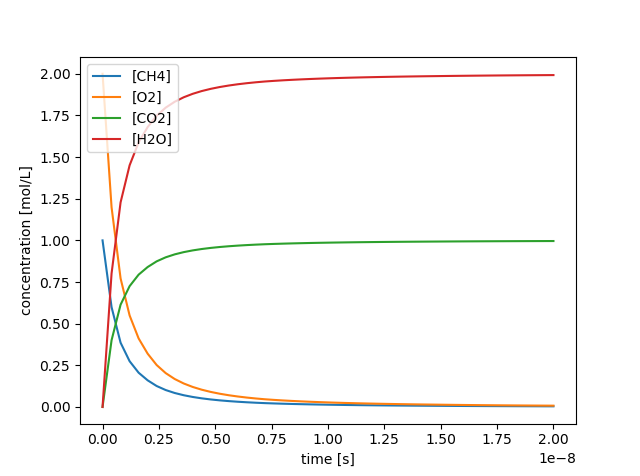
\includegraphics[width=\textwidth]{images/one-step-python.png}
        \caption{Python \parencite[p.~26]{methane_python}}
        \label{fig:one-step-python}
    \end{subfigure}
    \caption{One-step mechanism of methane combustion}\label{fig:one-step}
\end{figure}

\section{Two-step mechanism}

The combustion of methane is actually a sequence of elementary reactions rather than the straightforward one-step mechanism. The 2S\_CH4\_BFER scheme by \textcite{FRANZELLI2012621} considered in this section is explained in subsection~\ref{subsec:CO}. We would like to find an approximation solution to the following model for $0 < t < 10^{-7}$.
\begin{subequations}
\begin{align}
    \frac{\mathrm d [\ce{CH4}]}{\mathrm d t} &= - k_1 , \\
    \frac{\mathrm d [\ce{O2}]}{\mathrm d t} &= - 1.5k_1 - 0.5k_2 , \\
    \frac{\mathrm d [\ce{CO}]}{\mathrm d t} &= k_1 - k_2 , \\
    \frac{\mathrm d [\ce{CO2}]}{\mathrm d t} &= k_2 , \\
    \frac{\mathrm d [\ce{H2O}]}{\mathrm d t} &= 2k_1 .
\end{align}
\end{subequations}

The same parameters in table~\ref{tab:CO_k} on page~\pageref{tab:CO_k} are applied. We begin from the simulation with the initial conditions in table~\ref{tab:two-step-inputs} to compare the solutions with the existing Python implementation. 

\begin{table}[ht!]
\centering
\begin{tabular}{l c} 
 \hline
 Species & Initial values \\
 \hline
 \ce{CH4} & 1.0 \\
 \ce{O2} & 2.0 \\
 \ce{CO} & 0.0 \\
 \ce{CO2} & 0.0 \\
 \ce{H2O} & 0.0 \\
 \hline
\end{tabular}
\caption{Inputs for the two-step reaction mechanism of methane combustion}
\label{tab:two-step-inputs}
\end{table}

\begin{figure}[ht!]
    \centering
    \begin{subfigure}[b]{0.38\textwidth}
        \includesvg[width=\textwidth]{images/two_step_mechanism_methane}
        \caption{Julia}
        \label{fig:two-step-julia}
    \end{subfigure}
    ~ %add desired spacing between images, e. g. ~, \quad, \qquad, \hfill etc. 
      %(or a blank line to force the subfigure onto a new line)
    \begin{subfigure}[b]{0.58\textwidth}
        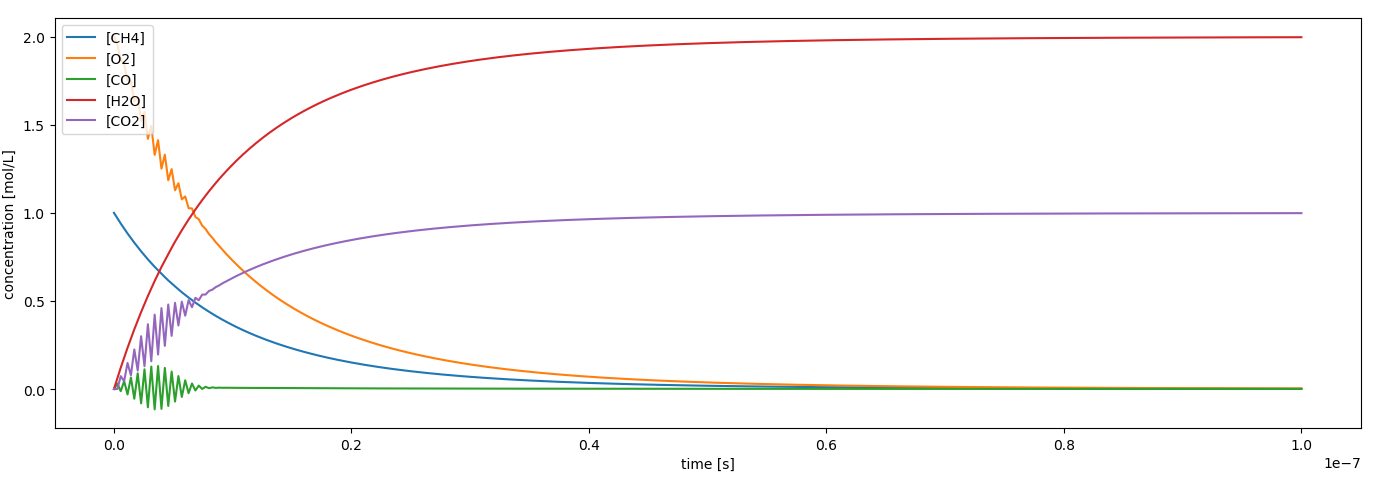
\includegraphics[width=\textwidth]{images/two-step-python.png}
        \caption{Python \parencite[p.~28]{methane_python}}
        \label{fig:two-step-python}
    \end{subfigure}
    \caption{Two-step mechanism of methane combustion}\label{fig:two-step}
\end{figure}

The results in figure~\ref{fig:two-step} look the same for both implementations except the small fluctuation in Python's figure~\ref{fig:two-step-python} due to the numerical methods it adopted. Note that while we are investigating pollutant formation, it is not particularly obvious from the figure that the carbon monoxide (\ce{CO}) is produced. Figure~\ref{fig:two-step-CO} is a separate graph for \ce{CO}. The concentration of \ce{CO} jumps sharply away from 0 immediately after the reaction starts.

\begin{figure}[ht!]
    \centering
    \includesvg[width=0.8\textwidth]{images/two_step_mechanism_methane_CO}
    \caption{Carbon monoxide in two-step mechanism of methane combustion}
    \label{fig:two-step-CO}
\end{figure}
\chapter{Chemical reaction network with Julia} \label{ch:network}

{\large \color{red} TODO}

\section{Problem definition}

\section{Examples}

\subsection{5-node 5-edge network with main flux and~recirculation}

\subsection{5-node 5-edge network with main flux and by-pass}

\section{Jacobian matrix}

\section{Performance}
\chapter{Conclusion} \label{ch:conclusion}

The research was initiated with the growing demand for a computational tool that is able to simulate large chemical reaction networks and to predict pollutant emission. We applied the Julia programming language to solve the one- and the two-step mechanism of methane combustion, the 5-node-5-edge networks and larger line-shaped networks. 

The results of performance measurement prove that Julia with its ecosystem is competent in simulating large network dynamics within reasonable time as long as appropriate numerical solvers are chosen. However, unlike C/C++ and Python, Julia has a rather shorter history. The Julia core code and its packages are still under heavy development thanks to the common effort from the open-source Julia community. It can be foreseen that Julia will be shortly utilized to speed up CRN simulations in industry and to estimate emissions more accurately for industrial furnaces.

%% This defines the bibliography file (main.bib) and the bibliography style.
%% If you want to create a bibliography file by hand, change the contents of
%% this file to a `thebibliography' environment.  For more information 
%% see section 4.3 of the LaTeX manual.

\begin{singlespace}
\printbibliography[heading=bibintoc]
\end{singlespace}


\appendix

\definecolor{LightGray}{gray}{0.95}
\definecolor{codegreen}{rgb}{0,0.6,0}
\definecolor{codegray}{rgb}{0.5,0.5,0.5}
\definecolor{codepurple}{rgb}{0.58,0,0.82}
\definecolor{backcolour}{rgb}{0.95,0.95,0.92}

\chapter{Julia implementation}

Listing~\ref{lst:project.toml} shows the project dependencies. The Julia language and the packages in other versions are not tested.

\begin{listing}[ht]
\inputminted[
    frame=lines,
    framesep=2mm,
    baselinestretch=1.2,
    bgcolor=LightGray,
    fontsize=\footnotesize,
    linenos
]{bash}{code/Project.toml}
\caption{Project dependencies}
\label{lst:project.toml}
\end{listing}

\begin{listing}[ht]
\inputminted[
    frame=lines,
    framesep=2mm,
    baselinestretch=1.2,
    bgcolor=LightGray,
    fontsize=\footnotesize,
    linenos
]{julia}{code/one_step_methane.jl}
\caption{One-step reaction mechanism of methane combustion}
\label{lst:one-step}
\end{listing}


\end{document}

